\documentclass{mipt-thesis-bs}
% Следующие две строки нужны только для biblatex. Для inline-библиографии их следует убрать.
%\usepackage{mipt-thesis-biblatex}
\usepackage[ruled,vlined]{algorithm2e}
%\addbibresource{example.bib}
\usepackage{graphicx}
\usepackage{subfigure}

\title{Обучение с подкреплением с применением экспертных демонстраций}
\author{Айтыгулов Э.}
\supervisor{Осипов Г.\,С.}
%\referee{Петров Д.\,Е.}       % требуется только для mipt-thesis-ms
\groupnum{М05-878б}
\faculty{Физтех-школа Прикладной Математики и Информатики}
\department{Кафедра системных исследований}

\begin{document}

\frontmatter
\titlecontents

\chapter{Введение}
Обучение с подкреплением - быстро прогрессирующая область машинного обучения, которая позволяет решать различные задачи управления в пространствах состояния большой размерности. Используя современные методы оптимизации и аппроксимации были получены внушительные результаты: \cite{Agent-57} переигрывает человека в 57 играх Atari 2600; \cite{OpenAI}  обучили ботов способных обыграть команду профессиональных игроков в многопользовательской игре Dota2; бот обученный в \cite{DeepMind} смог получить статус <<GrandMaster>> в онлайн игре StarCraft2, а это значит, что он обыгрывает $99.8\%$ игроков по всему миру. Однако, несмотря на успехи, обучение с подкреплением имеет ряд проблем, из-за которых оно не может быть применено в широком круге задач. Одна из таких проблем - необходимость большого количества взаимодействий со средой и поведение агента в начале обучение, которое далеко от идеального . Все это не позволяет применять обучение с подкреплением на реальных или сложных задачах. Для решения этих проблем могут быть использованы экспертные демонстрации и симуляторы. Использование демонстраций и адаптация моделей, обученных в симуляторе, к реальному миру - одни из самых перспективных направлений.

Цель данной работы применение методов обучения с подкреплением в задаче управления робототехническим манипулятором в симулляторе. В работе исследуются методы по работе с <<неидеальными>> демонстрациями, т.к. это может быть использовано для ускорения процесса обучения и уменьшения затрачиваемых ресурсов для моделей, работающих с изображениями в качестве входных данных, с помощью моделей использующих данные доступные в симуляторе. 

Данный подход может быть применен в задачах по переносу моделей из симулятора в реальность, когда модель, обученная в симуляторе, с помощью техник рандомизации или домен адаптации переносится на реального робота.

В качестве базовых алгоритмов использовались асинхронный алгоритм Ape-X DQN и улучшенная версия Ape-X DDPG  \cite{apex}. В качестве рабочей среды было реализовано окружение использующее симулятор CoppeliaSim.

\mainmatter
\chapter{Обучение с подкреплением}

Обучение с подкреплением - способ обучения модели с помощью ее взаимодействия с некоторой окружающей средой, в которой она совершает действия, наблюдает ее состояния и получает положительный или отрицательный отклики (подкрепление). Алгоритмы обучения с подкреплением нацеленны на увеличение суммарной награды.

\section{Марковский процесс принятия решений}
Для описания всей системы используется марковский процесс принятия решений (рис.\ref{mdp}). В каждый момент времени t=0, 1, 2, 3... агент, находясь в состоянии $s_t\in S$ может совершать некоторое $a_t\in A$, за что получает вознаграждение $R_t$ с вероятностью $P(R_{t+1}|s_t,a_t)$. В ответ на действие $a_t$ окружение переходит в некоторое состояние $s'_t$ с вероятностью $P(s_{t+1}|s_t,a_t)$. Функция распределения $P$, должна обладать следующим свойством:

$P(s_{t+1}, R_{t}|s_t,a_t,s_{t-1},a_{t-1}) = P(s_{t+1}, R_{t}|s_t,a_t)$

Это свойство называется Марковским свойством. Оно означает, что динамика среды полностью описывается функцией распределения $P$ и что состояние $s_t$ содержит всю информацию определяющую следующие состояния системы. Используя $P$ можно посчитать математическое ожидание величины $R$:

$r(s, a) = \mathbb{E}[R_{t} | s_t, a_t]=\sum_{R \sim P} R \sum_{s_{t+1} \in S} P(s_{t+1}, R | s_t, a_t)$

Модель поведения агента описывается вероятностным распределением $\pi$. В состоянии $s$ агент выбирает действие $a$ с вероятностью $\pi(a|s)$. Цель агента увеличение суммарной награды за эпизод. Во избежании расходимости ряда вводится дисконтирующий фактор $0 \leq\gamma\leq 1$:

$G_{t} = R_{t+1}+\gamma R_{t+2}+\gamma^{2} R_{t+3}+\cdots=\sum_{k=0}^{\infty} \gamma^{k} R_{t+k+1}$

Кроме ограничения величины $G$ дисконтирующий фактор $\gamma$ также определяет что важнее для агента: максимизировать сиюминутную награду (в случае $\gamma$ близкого к нулю) или кумулятивную (в случае $\gamma$ близкого к единице).

%рисунок МППР
\begin{figure*}[ht]
    \centering
    \subfigure{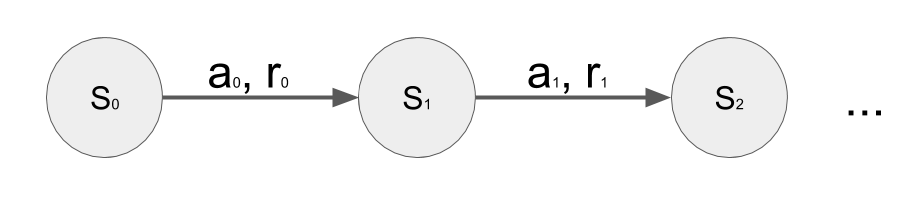
\includegraphics[width=0.5\linewidth]{img/mdp.png}}
    \vspace{-0.2cm}
    \caption{Марковский процесс принятия решений}
    \label{mdp}
\end{figure*}

\section{Функции ценности}

Большинство алгоритмов для оценки или улучшения стратегии так или иначе используют функции ценности - функции, которые оценивают величину $G$ при условии некоторого состояния $s$ или некоторого действия $a$ в состоянии $s$ с учетом текущей стратегии:

Функция ценности состояния: $V_{\pi}(s_t) = \mathbb{E}_{\pi}[G_{t} | s_t]=\mathbb{E}_{\pi}[\sum_{k=0}^{\infty} \gamma^{k} R_{t+k+1} | s_t]$ 
 
Функция ценности действия: $Q_{\pi}(s_t, a_t) = \mathbb{E}_{\pi}[G_{t} | s_{t}, a_{t}]=\mathbb{E}_{\pi}[\sum_{k=0}^{\infty} \gamma^{k} R_{t+k+1} | s_{t}, a_{t}]$

$V_\pi$ и $Q_\pi$ оценивают математическое ожидание суммарного вознаграждения, полученного до конца эпизода, при условии текущего состояния $s_t$ или действия $a_t$ в состоянии $s_t$ при условии следования далее стратегии $\pi$. Из определения функций ценности следуют следующие равенства (уравнения Беллмана):
\begin{center}
(1.1) $V_{\pi}(s_t) = \mathbb{E}_{\pi}[G_t | s_t]=\mathbb{E}_{\pi}[R_{t} + \gamma G_{t+1}| s_t] = \mathbb{E}_{\pi}[R_{t} + \gamma V_{\pi}(s_{t+1})| s_t]$ 

(1.2) $Q_{\pi}(s_t, a_t) = \mathbb{E}_{\pi}[G_{t} | s_t, a_t]=\mathbb{E}_{\pi}[R_{t} + \gamma G_{t+1}| s_t, a_t] = \mathbb{E}_{\pi}[R_{t} + \gamma V_{\pi}(s_{t+1})| s_t, a_t]$
\end{center}

Решение задачи обучения с подкреплением подразумевает поиск стратегии, которая получала положительных откликов среды больше какой либо другой стратегии. Функция ценности $V$ позволяет это сделать:

\begin{center}
    $\pi \geq \pi' \Rightarrow \forall s \in S \hookrightarrow V_\pi(s) \geq V_{\pi'}$
\end{center}

$Q^*$ и $V^*$ обозначают функции ценности соответствующие $\pi^*= argmax_{\pi} V_\pi$

\section{Q-обучение}

В данной работе использовались два алгоритма обучения с подкреплением: DQN \cite{dqn} и TD3 \cite{td3}. Первый алгоритм работает с дискретным пространством действий, а второй с непрерывным. Оба алгоритма основаны на табличном методе поиска оптимальной стратегии - Q-обучение \cite{Q-learning}. Алгоритм представляет из себя итеративный процесс, который в МППР с конечным множеством $S$ и конечным множеством $A$ находит оптимальную стратегию $\pi^*$. Идея подхода лежит в использовании уравнений Беллмана для оптимальной стратегии:
\begin{center}
$Q_{\pi^*}(s_t, a_t) = \mathbb{E}_{\pi^*}[R_{t} + \gamma V_{\pi^*}(s_{t+1})| s_t, a_t]$

$V_{\pi^*}(s_t) = \max_{a\in A}Q_{\pi^*}(s_t, a)$
\end{center}

Грубо говоря, уравнения Беллмана значат, что если известна функция $Q_{\pi^*}$, то, чтобы стратегия была оптимальной, нужно выбирать действия с наибольшим значением $Q_{\pi^*}$ в каждом состоянии. Q-обучение использует этот факт для обновления стратегии, для которой на каждом шаге оценивает функцию $Q$ с помощью динамического программирования: 

\begin{algorithm}[H]
\SetAlgoLined
Initialize $Q(s, a)$ with zeros\;
 \While{current episode < max_episode}{
  Initialize $s$\;
  Initialize done=False\;
  \While{not done}{
  Choose $a$ for $s$ using $Q$ (e.g. $\epsilon$-greedy)\;
  Act $a$, observe $R, s', done$\;
  $Q(s, a) \leftarrow Q(s, a)+\alpha[R+\gamma \max _{a'} Q(s', a')-Q(s, a)]$\;
  $s \leftarrow s'$\;
  }
 }
\caption{Q-обучение}
\end{algorithm}

На каждом шаге действие выбирается с учетом текущего значения $Q$ и стратегии исследования, которая необходима, чтобы не сойтись к суб-оптимальному решению. В большинстве случаев используется $\epsilon$-жадная стратегия: с вероятностью $\epsilon$ выбирается случайное действие, а в остальных случаях $argmax_aQ(s,a)$. Разница $R+\gamma \max _{a'} Q(s', a')-Q(s, a)$ называется TD-ошибкой.

\chapter{Обзор Работ}

% \let\clearpage\relax 
\chapter{Используемые методы}
\section{DQN}

Большинство задач имеют непрерывное пространство $S$ большой размерности, что делает классический вариант Q-обучения непригодным. Однако современные вычислительные возможности и методы оптимизации позволяют вместо таблицы $Q(s,a)$ использовать аппроксиматор $Q_\theta$ с обучаемыми параметрами $\theta$. Например в работе \cite{dqn}, где такой подход использовался впервые, в качестве аппроксиматора выступает сверточная нейронная сеть. Ключевые элементы алгоритма, которые позволили использовать аппроксиматор: реплэй-буфер $D$ и таргет-копия аппроксиматора с параметрами $\theta'$, которые периодически заменялись параметрами $\theta$ основного аппроксиматора. Параметры $\theta$ настраивались с помощью оптимизации  целевого функционала $L$ одним из градиентных методов. в качестве $L$ может выступать среднеквадратичная ошибка:

\begin{center}
    
$L(\theta)=\frac{1}{N}\sum_{(s,a,r,s,d) \sim D} (Q_\theta(s, a) - target)$,

где $target = r + \gamma\cdot d \cdot Q_{\theta'}(s',argmax_{a'}Q_{\theta'}(s',a'))$,

$N$ - размер выборки.
\end{center}

\section{Стабилизация целевой переменной и оптимизация архитектуры аппроксиматора}

В работе \cite{double dqn} было показано, что проблема такого подхода в том, что целевая величина переоценивает значение $Q$. Авторы предлагают для стабилизации разделить выбор действия и оценку $Q$ с помощью таргет-копии:

\begin{center}
$target = r + \gamma\cdot d \cdot Q_{\theta'}(s',argmax_{a'}Q_{\theta}(s',a'))$ 
\end{center}

Также для уменьшения дисперсии в \cite{n-step} к TD-ошибке добавляют nTD-ошибку:

\begin{center}
$L_n(\theta)=\frac{1}{N}\sum_{(s,a,r,s,d) \sim D} (Q_\theta(s, a) - target_n)$,

где $target_n = \sum_{i=0}^{n}\gamma^i\cdot r_i + \gamma^n\cdot d_n \cdot Q_{\theta'}(s_n,argmax_{a_n}Q_{\theta'}(s_n,a_n))$,

$N$ - размер выборки.
\end{center}

Для ускорения сходимости авторы \cite{dueling dqn} предлагают, использовать величину $A(s,a)=Q(s,a) - V(s)$. В работе вместо одного аппроксиматора для величины $Q$ используются аппроксиматоры для $V$ и для $A$, значения которых далее суммируются. Такая архитектура позволяет не исследовать состояние $s$ и не тратить время на оценку $Q(s,a)$.

\section{Приоритезированный буфер}

Реплэй буфер позволяет накапливать и пере-использовать опыт прошлых взаимодействий со средой. Все элементы буфера могут быть использованы на текущей итерации с одинаковой вероятностью. Такой подход игнорирует разницу в сэмплах и не учитывает, что некоторые элементы могут быть намного важнее остальных, но в то же время могут быть очень редкими. В \cite{per} используют приоритизацию для ускорения обучения. Вероятность сэмпла тем больше, чем выше модуль ошибки модели на этом сэмпле.

Для сэмпла $i$ вводится величина $p_i=|\delta_i| + \epsilon$, где $\delta_i$ - ошибка модели, а $\epsilon$ - константа близкая к нулю, необходимая для ограничения $p_i$ снизу. Вероятность вычисляется по следующей формуле:

\begin{center}
    $P(i)=\frac{p_{i}^{\alpha}}{\sum_{k} p_{k}^{\alpha}}$
\end{center}

С помощью константы $\alpha$ контролируется степень приоритизации: чем меньше $\alpha$, тем ближе вероятностное распределение к равномерному. Чтобы оценка математического ожидания соответствовала действительному распределению, каждый сэмпл входит в целевой функционал с обратно пропорциональным весом (Imortance Sampling):

\begin{center}
$w_{i}=\left(\frac{1}{N} \cdot \frac{1}{P(i)}\right)^{\beta}$    
\end{center}

Чем выше $\beta$, тем больший вклад делает каждый сэмпл. Одновременное увеличение $\beta$ и $\alpha$ увеличивает степень приоритизации

\section{Использование демонстраций}

В качестве расширения \cite{dqn}, которое бы позволило эффективно использовать демонстрации, был выбран алгоритм, предложенный в \cite{dqfd} с модифицированным буфером ForgER. Алгоритм комбинирует обучение с подкреплением и обучение с учителем и состоит из двух частей: пред-обучение на экспертных данных и дообучение в среде. Экспертные данные добавляются в буфер с более высоким приоритетом и остаются там до конца обучения. 

Т.к. в демонстрациях представлены только экспертные действия, то значения $Q$ известны тоже только для экспертных действий. Чтобы значения остальных действий не были произвольными используется добавка к целевому функционалу, которая ограничивает их значения:

\begin{center}
    $J_{E}(Q)=\max _{a \in A}[Q(s, a)+l(a_{E}, a)]-Q(s, a_{E})$,
    
    где $l(a_{E}, a) = 0$, если $a_{E} = a$, и константа $margin>0$ в ином случае
\end{center}
 
 
\section{ForgER}

В классическом алгоритме демонстрации не удаляются из буфера, но это не сказывается на обучении только в случае хороших демонстраций. На практике демонстрации могут быть записаны суб-оптимальной стратегией, записаны в других условиях и т.д.. Одним из таких примеров является изменение пространства действий: при решении некоторых задач производится дискретизация непрерывного пространства $A$, после которой итоговое пространство действий становится конечным, и т.о. дискретизация экспертных действий приводит к потери некоторой доли информации.  Это может привести к переобучению и суб-оптимальному поведению. По этой причине в буфере ForgER добавлена возможность удаления данных.

Скорость забывания контролируется параметром $d$ и номера текущего эпизода $k$:

\begin{center}
    $proportion_{demo} = \min(1, k/d)$
\end{center}

% \let\clearpage\relax
\section{TD3}

Для работы с непрерывным множеством действий $A$ широко используются алгоритмы основанные на детерминированном градиенте стратегии. В отличии от конечных множеств действий, где максимум аппроксимации $Q$ можно найти перебрав значения, в непрерывном множестве действий так сделать нельзя. Один из подходов для решения этой задачи - использования актор-критик архитектуры. В дополнении к апроксиматору $Q(s,a)$, который исполняет роль критика и параметризован весами $\theta^Q$, используется второй аппроксиматор $\mu:S\rightarrow A$, который исполняет роль актора и с помощью которого выбираются действия. Т.о. стратегия агента параметризуется весами $\theta^\mu$. Теорема о детерминированном градиенте стратегии позволяет оптимизировать $\theta^\mu$ с помощью градиентных методов. Целевым функционалом для оптимизации является $J(\mu)=\mathbb{E}_{s\sim P, a\sim\mu}G_0$ и теорема говорит, что градиент $J$ равен математическому ожиданию произведения градиента $Q$ по $\mu$ и градиента $\mu$:

\begin{center}
$\nabla_{\theta^\mu} J(\mu) =\mathbb{E}_{s \sim P}[\nabla_{\theta^\mu} \mu(s) \nabla_{a} Q^{a}(s, a)|_{a=\mu(s)}]$
\end{center}

На практике, чтобы обучение было более стабильным, также используются таргет-копии аппроксиматоров. В работе \cite{ddpg}, вместо периодического копирования весов используется усреднение Поляка \cite{polyak}:

\begin{center}
    $\theta^{\mu^{\prime}} \leftarrow \tau \theta^{\mu}+(1-\tau) \theta^{\mu^{\prime}}$
    
     $\theta^{Q^{\prime}} \leftarrow \tau \theta^{Q}+(1-\tau) \theta^{Q^{\prime}}$
\end{center}

\section{Сглаживание апроксимации функции значимости}

Проблема переоценки некоторых действий в начале обучения при использовании аппроксиматоров функции значимости также присутствует в актор-критик архитектуре. Если критик в состоянии $s$ имеет сильно выраженный максимум в некоторой точке $a\in A$, то этот максимум используется актором, что делает обучение более сложным. Данную проблему решают в работе \cite{td3}.

Во-первых частота обновлений параметров $\theta^\mu$ и параметров $\theta^{\mu'}, \theta^{Q'}$ таргет аппроксиматоров уменьшается по сравнению с частотой обновлений $\theta^Q$, чтобы TD-ошибка не аккумулировалась в таргет аппроксиматорах. Т.о задержка между обновлениями улучшает сходимость алгоритма.

Во-вторых оценка целевой переменной ограничивается сверху. Для этого используется второй аппроксиматор $Q_twin$, а к действиям добавляется гауссовский шум:

\begin{center}
    $a'(s')=\operatorname{clip}(\mu'(s')+\operatorname{clip}(\epsilon,-c, c), a_{L o w}, a_{H i g h}), \quad \epsilon \sim \mathcal{N}(0, \sigma)$
    
    $target=r+\gamma(1-d) \min _{i=1,2} Q_i(s', a'(s')$
\end{center}

\section{Параметризованный шум для эффективного исследования среды}

В работах \cite{ddpg, td3} для исследования среды используется либо некоррелирующий гауссовский шум, либо коррелирующий гауссовский шум (случайный процесс Орнштейна-Уленбека). В работах \cite{noisy layers, adaptive noise} предлагается адаптивный метод исследования, представленный в виде модифицированного слоя нейронной сети. Адаптивный метод исследования позволяет не настраивать параметры шума, т.к. веса аппроксиматора сами подстраиваются под него с учетом окружающей среды, делая исследование более эффективным. 

Классический слой нейронной сети $y$ вычисляется через произведение матрицы:

\begin{center}
    $y=w x+b$,
\end{center}

где $x$ - входной слой, а $w$ и $b$ настраиваемые параметры. Адаптивный шум добавляется к каждому слою:

\begin{center}
    $y =(\mu^{w}+\sigma^{w} \odot \varepsilon^{w}) x+\mu^{b}+\sigma^{b} \odot \varepsilon^{b}$
\end{center}

Чтобы уменьшить время генерации случайных чисел, используется факторизированный шум: вместо генерации матрицы размером $p\times q$, где $p$ - размерность входного слоя, а $q$ - размерность выходного слоя, используются 2 случайных вектора $\varepsilon_i$ и $\varepsilon_j$ размерности $p$ и $q$. Матрица $\varepsilon^w$ и вектор $\varepsilon^b$ вычисляются следующим образом:

\begin{center}
$\varepsilon_{i j}^{w} =f(\varepsilon_{i}) f(\varepsilon_{j})$

$\varepsilon_{j}^{b} =f(\varepsilon_{j})$,

где $f(x)=\operatorname{sgn}(x) \sqrt{|x|}$
\end{center}

\section{Распределенные алгоритмы обучения с подкреплением}

Алгоритмам обучения с подкреплением для эффективного обучения требуется большое количество взаимодействий со средой, поэтому распределенные алгоритмы пользуются большой популярностью, т.к. при наличии вычислительных мощностей они позволяют ускорить набор необходимого опыта. В данной работе в качестве распределенной системы была выбрана архитектура Ape-X (рис.\ref{apex}) представленная в \cite{apex}.

Процесс обучения разбивается на 3 типа под-процессов: 1) <<Актор>> под-процессы, которые набирают опыт; 2) под-процесс <<Учитель>> , который оптимизирует параметры сети; 3) <<Буфер>> под-процесс, который добавляет накопленные данные в буфер, подготавливает их к обучению и обновляет приоритеты. При правильной настройке, под-процессы не ждут друг друга 

% рисунок Apex
\begin{figure*}[ht]
    \centering
    \subfigure{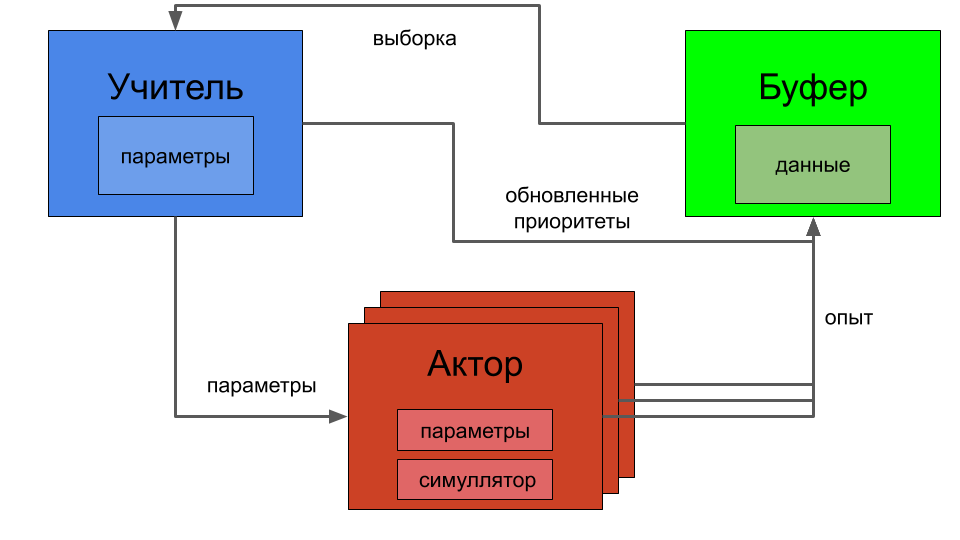
\includegraphics[width=0.5\linewidth]{img/apex.png}}
    \vspace{-0.2cm}
    \caption{Архитектура Ape-X}
    \label{apex}
\end{figure*}

<<Актор>> копируют параметры основного и таргет аппроксиматоров, накапливают опыт, вычисляют приоритеты на основе текущей копии параметров и отправляют его <<Буфер>> под-процессу. В случае конечного множества действий $A$ для эффективного исследования агенты используют $\epsilon$-жадную стратегию с разными параметрами $\epsilon$: агенты с большим $epsilon$ исследуют среду более широко, в то время как агенты с маленьким $\epsilon$ более глубоко. В случае непрерывного множества действий использовался некоррелированный гауссовский шум.

В экспериментах с окружением \textit{RozumEnv} в случае непрерывного множества действий использовался параметризованный шум представленный в \cite{noisy layers} и $\epsilon$-жадная стратегия для действия по сжатию манипулятора с разным $\epsilon$ для каждого агента. Параллельно под-процессу набирающим опыт, также работал под-процесс тестирующий среду с $\epsilon=0$

 
% \let\clearpage\relax
\chapter{Эксперименты}

В этой секции описываются детали проведенных экспериментов. Были проведены эксперименты показывающие важность забывания в разных окружениях и эксперименты по обучению робототехнического манипулятора в задаче по захвату предмета в дискретном и непрерывном множествах действий с использованием данных из симулятора в качестве состояний. 


\section{Изучение вклада забывания в обучающий процесс}

Для изучения вклада забывания были рассмотрены окружения:

1) сложные среда \textit{MineRLTreechop-v0} реализованная с помощью платформы \textit{Malmo}, позволяющая использовать игру \textit{MineCraft} для построения окружений;

2) набор окружений \textit{ClassicControl}: \textit{MountainCar-v0, CartPole-v0, Acrobot-v1};

3) набор окружений \textit{Box2D}: \textit{LunarLander-v2, CarRacing-v0}.

Окружение \textit{MineRLTreechop-v0} было реализовано в рамках соревнования \textit{MineRL}, как одно из вспомогательных окружений. Вместе с окружениями были собраны демонстрации для каждого из них. Цель агента научиться срубать блоки деревьев. За каждый блок агент получал $r=1$. В качестве $s$ выступала картинка размером 64x64. Пространство действий представляло из себя 8 действий, которые принимают значения \{0,1\} и два непрерывных действия по повороту камеры. Чтобы показать вклад забывания при изменении пространства действий были рассмотрены две дискретизации: 

1) с 7 действиями;

2) с 10 действиями - более аккуратная,

и 3 варианта забывания:

1) без забывания, с буфером предложенным в \cite{dqfd}

2) с частичным забыванием (минимальная пропорция демонстраций в выборке составляла 0.1)

3) с полным забыванием в течении 50 эпизодов

Как видно на рис.\ref{treechop}, чем больше меняется пространство действий, тем сильнее это сказывается на обучении. 

\begin{figure*}[ht]
    \centering
    \subfigure{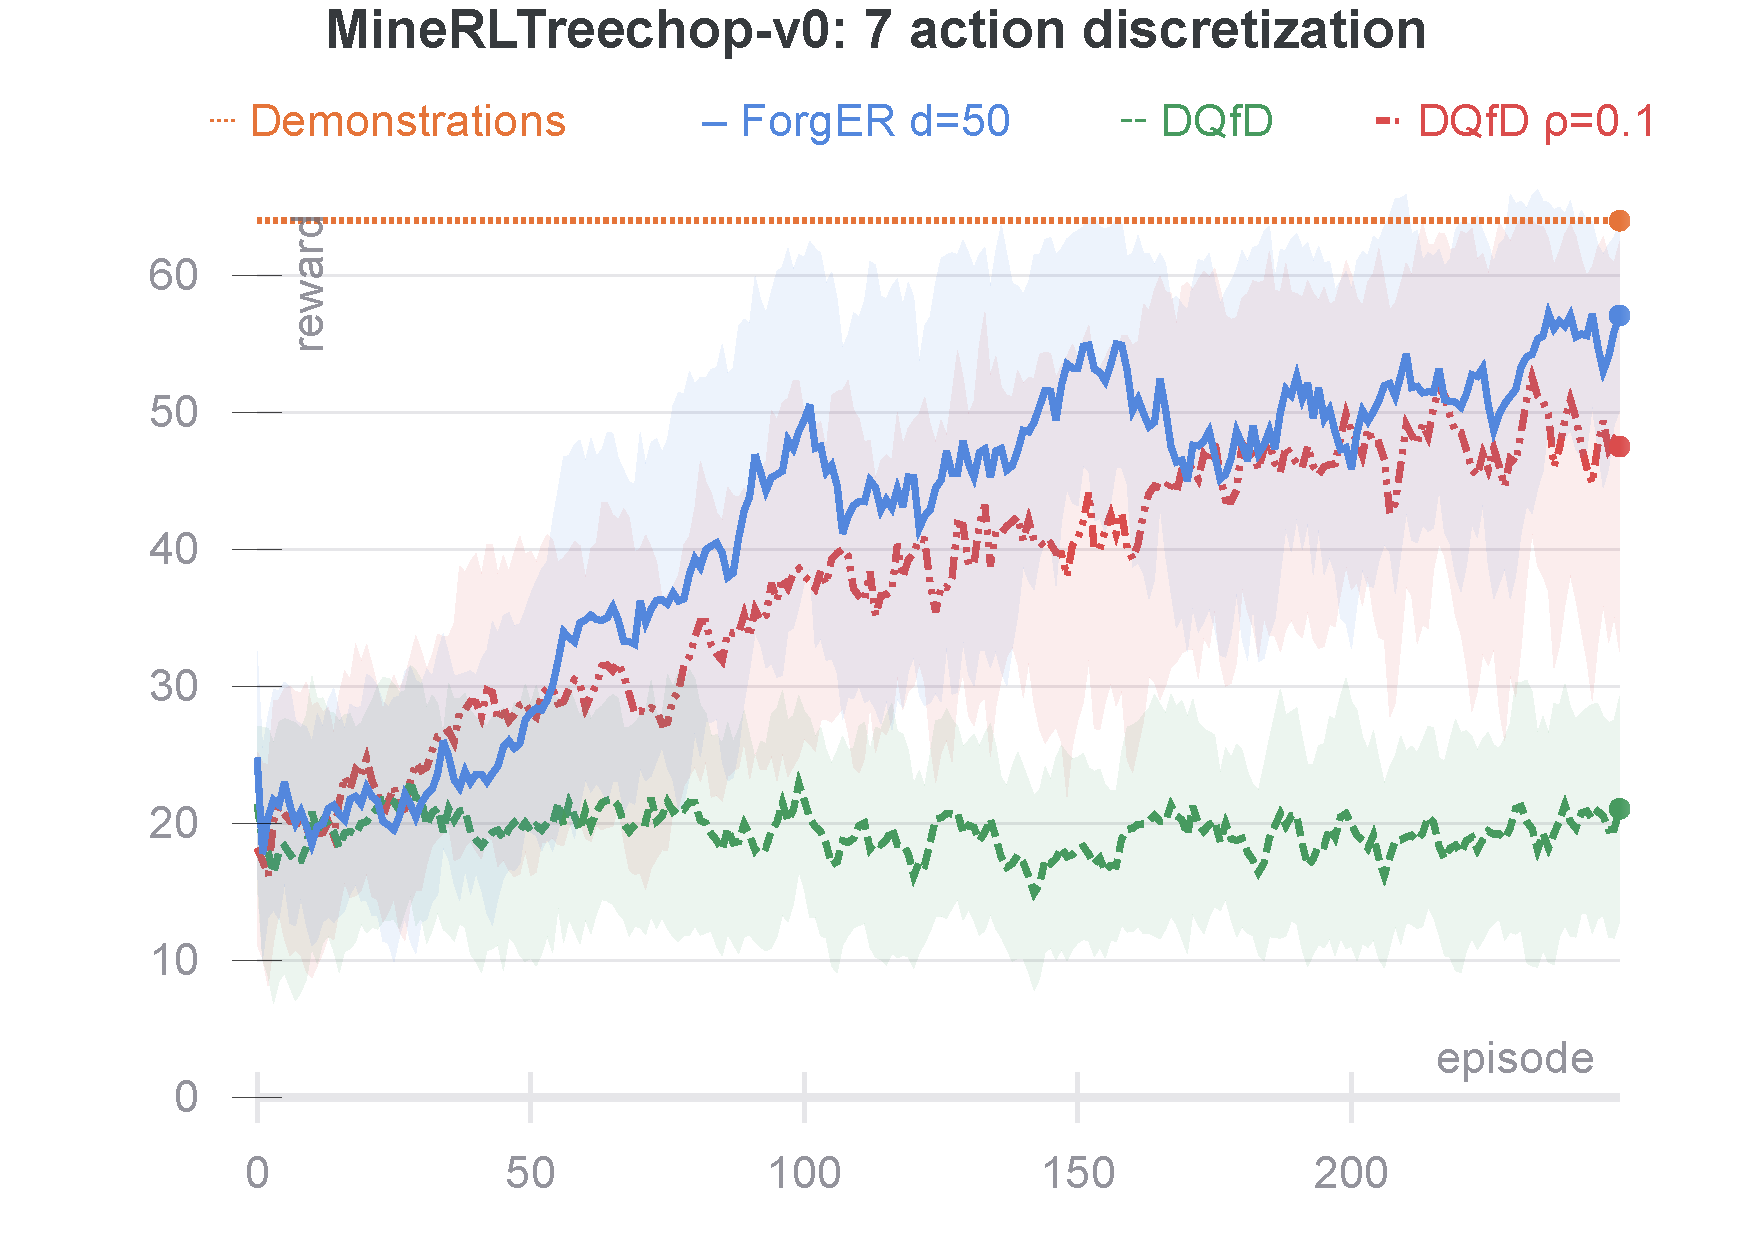
\includegraphics[trim={110px 20px 80px 50px},width=0.43\linewidth]{img/treechop/e2.pdf}}
    \hspace{0.08\linewidth}
    \subfigure{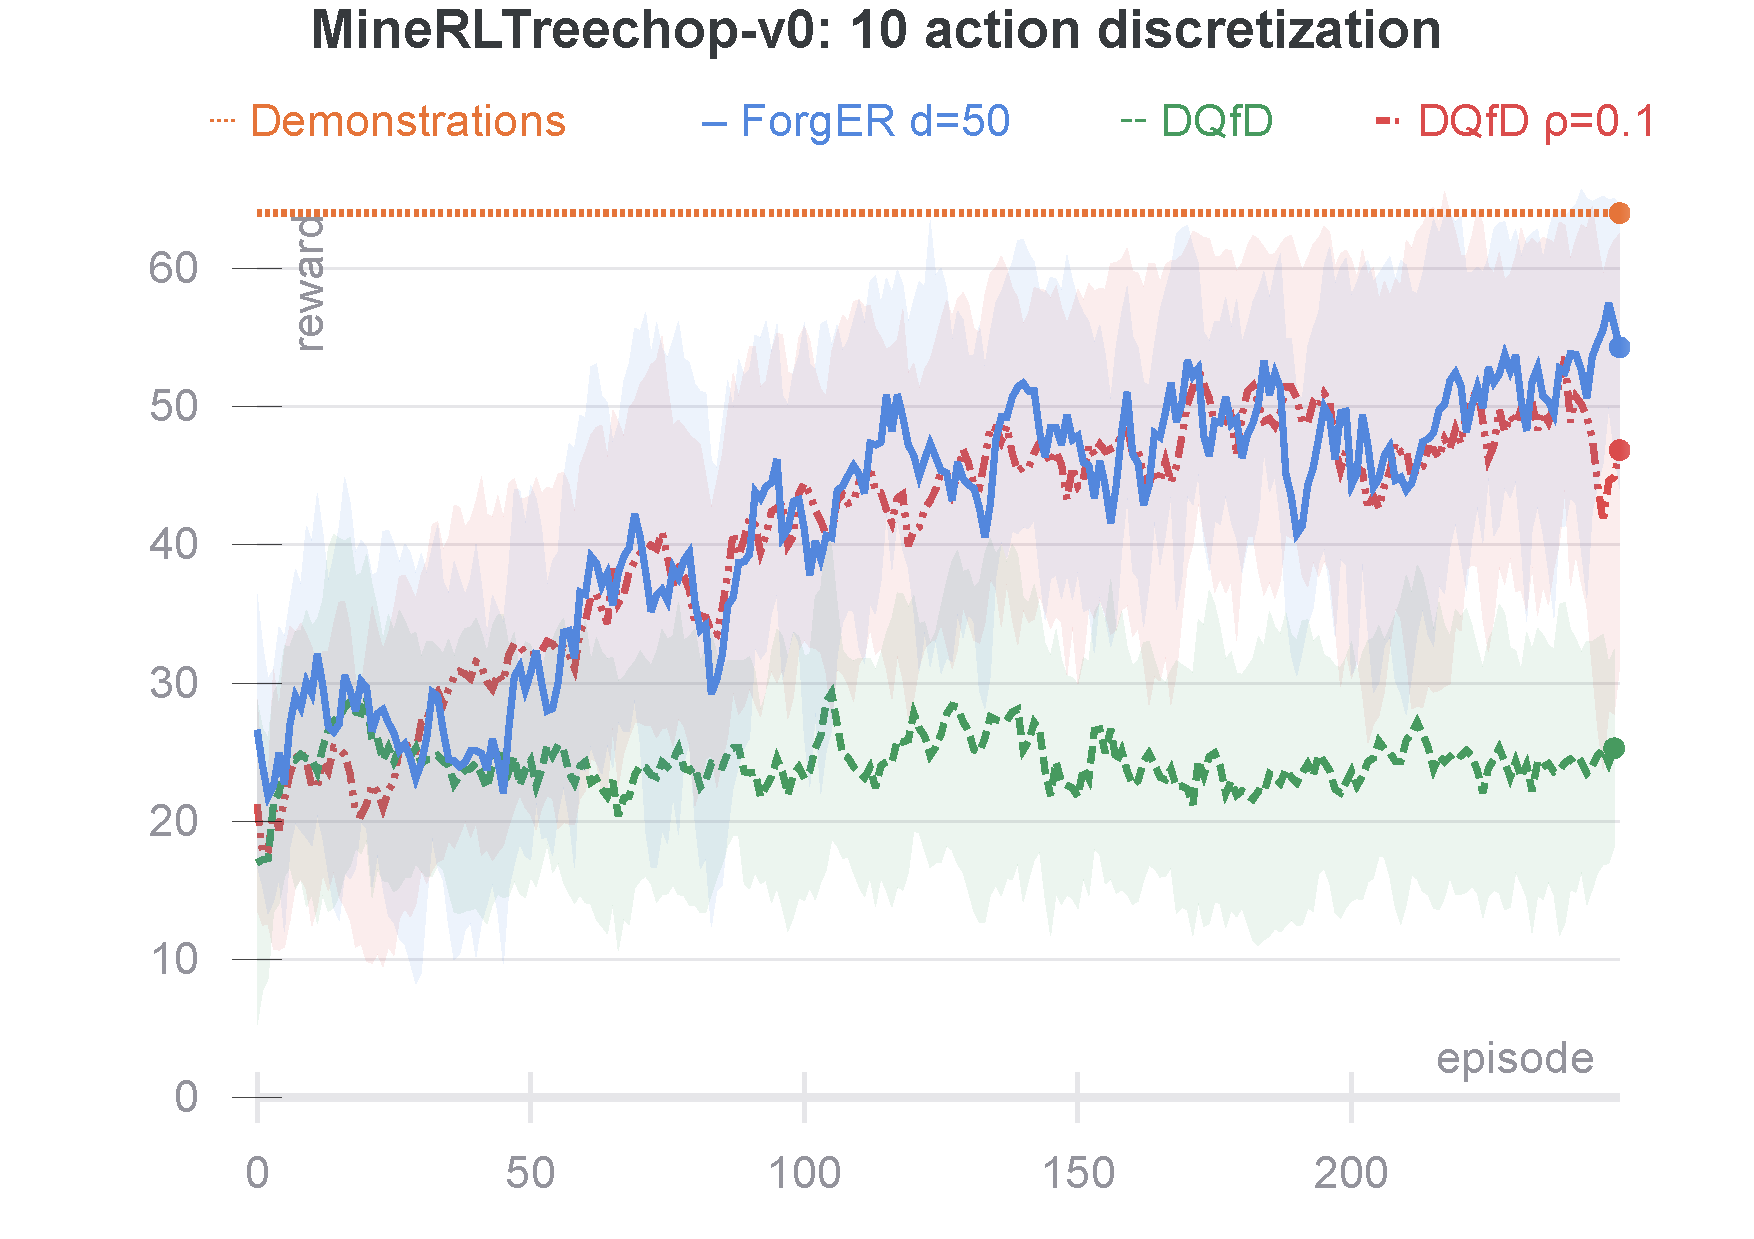
\includegraphics[trim={110px 20px 80px 50px},width=0.43\linewidth]{img/treechop/e1.pdf}}
    \vspace{-0.2cm}
    \caption{ \textbf{(Слева)} Средняя награда за эпизод при дискретизации с 7 действиями.
    \textbf{(Справа)} Средняя награда за эпизод при дискретизации с 10 действиями.
    \label{treechop}
    }
\end{figure*}

На наборе окружений \textit{ClassicControl} и \textit{Box2D} \textit{ForgER} был сравнен с алгоритмом \cite{pofd}, который показал хороший результат при работе с неидеальными демонстрациями. \textit{ClassicControl} - набор окружений с дискретными множествами действий и для каждого были собраны данные с низкими и высокими средними наградами. \textit{Box2D} - окружения с непрерывными множествами действий и данные имели высокую среднюю награду, но действия дискретизировались при записи. Для каждого окружения и набора данных был произведен поиск оптимального значения ключевых параметров и усреднение по 4 запускам. В первом случае ForgER показал сравнимые результаты на данных хорошего качества, и полностью уступил на данных плохого качества. Однако во втором случае, несмотря на демонстрации с большой средней наградой, дискретизация сильно сказалась на процессе обучения \cite{pofd}.  

\begin{figure*}[ht]
    \centering
    \subfigure{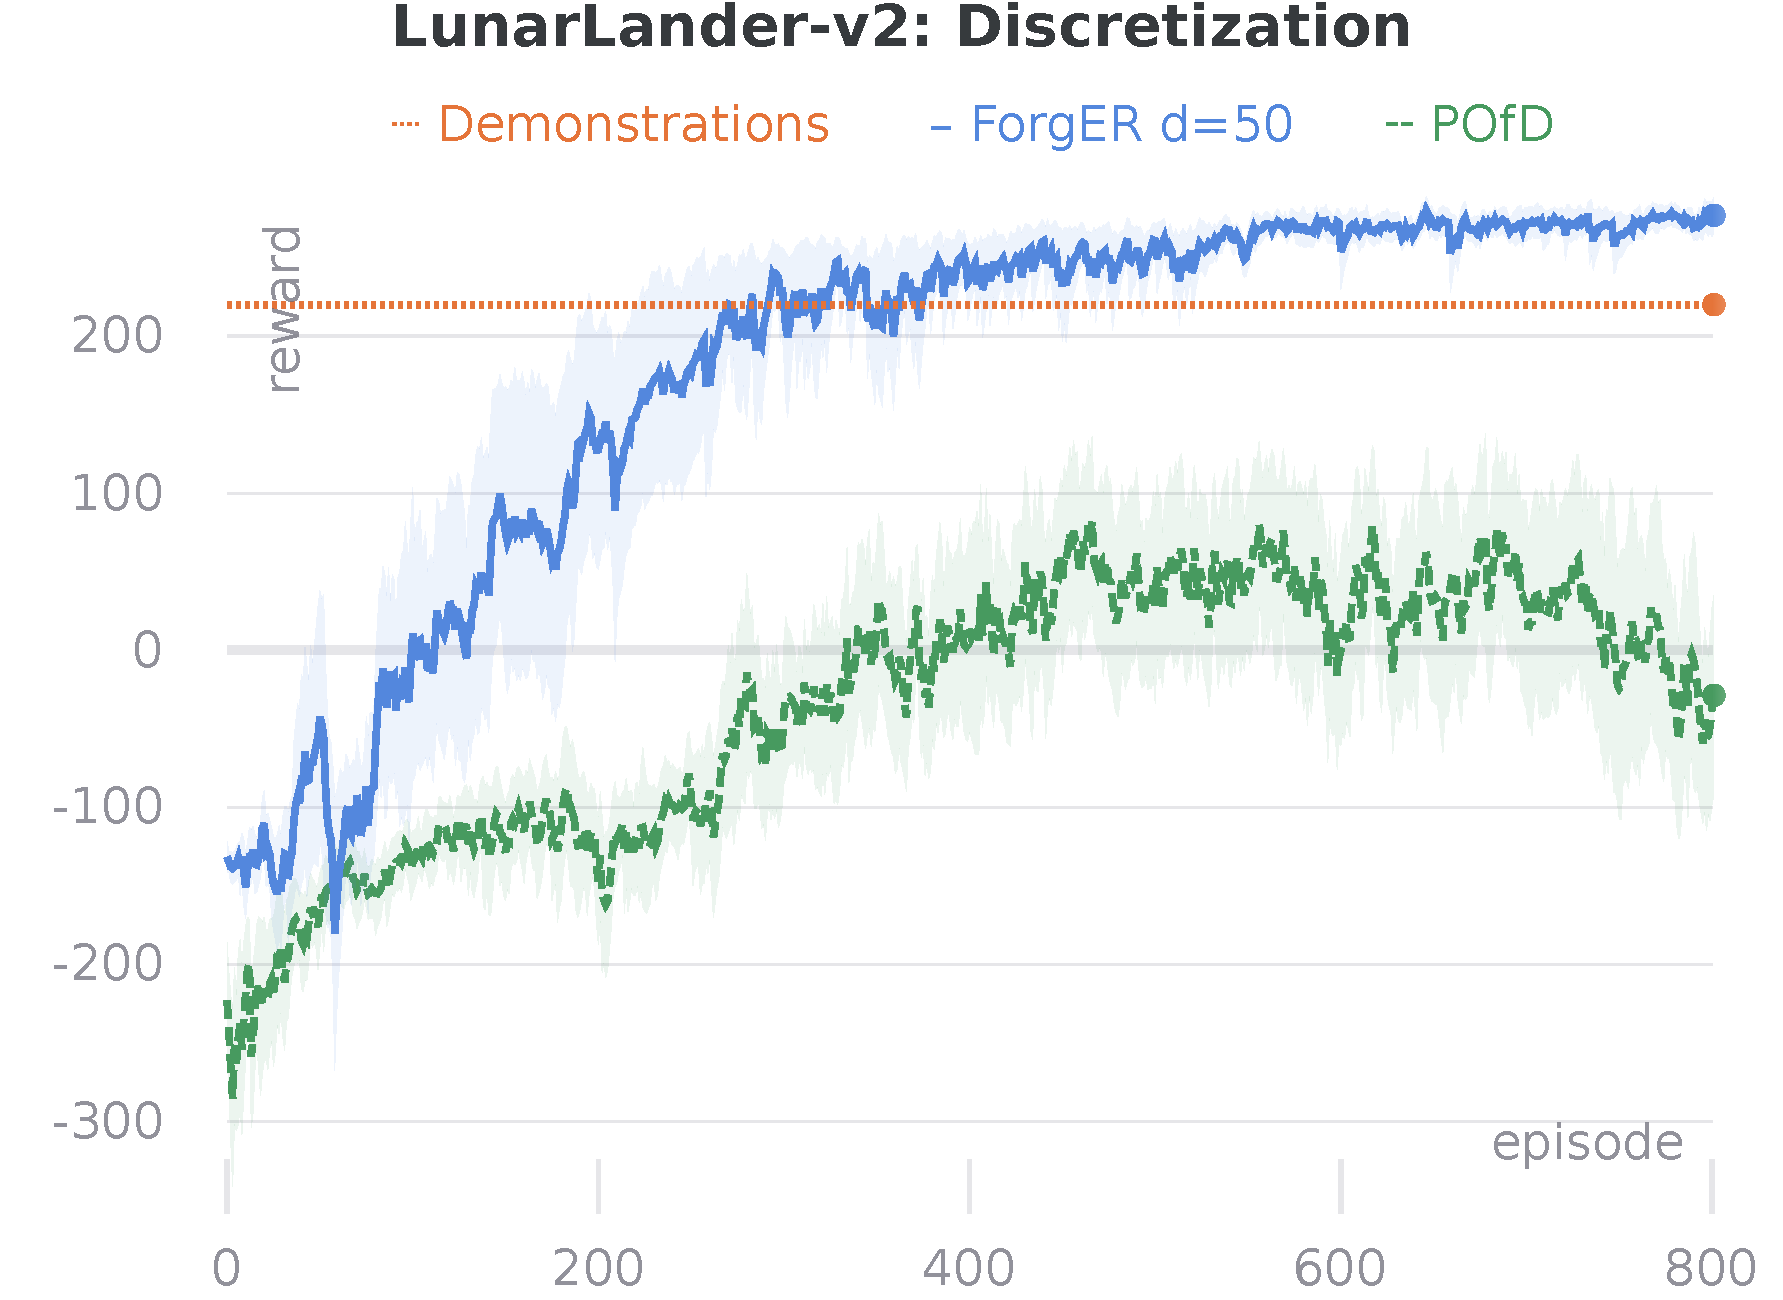
\includegraphics[width=0.48\linewidth]{img/discretization-lander-carracing/lander.pdf}}
    \hspace{0.02\linewidth}
    \subfigure{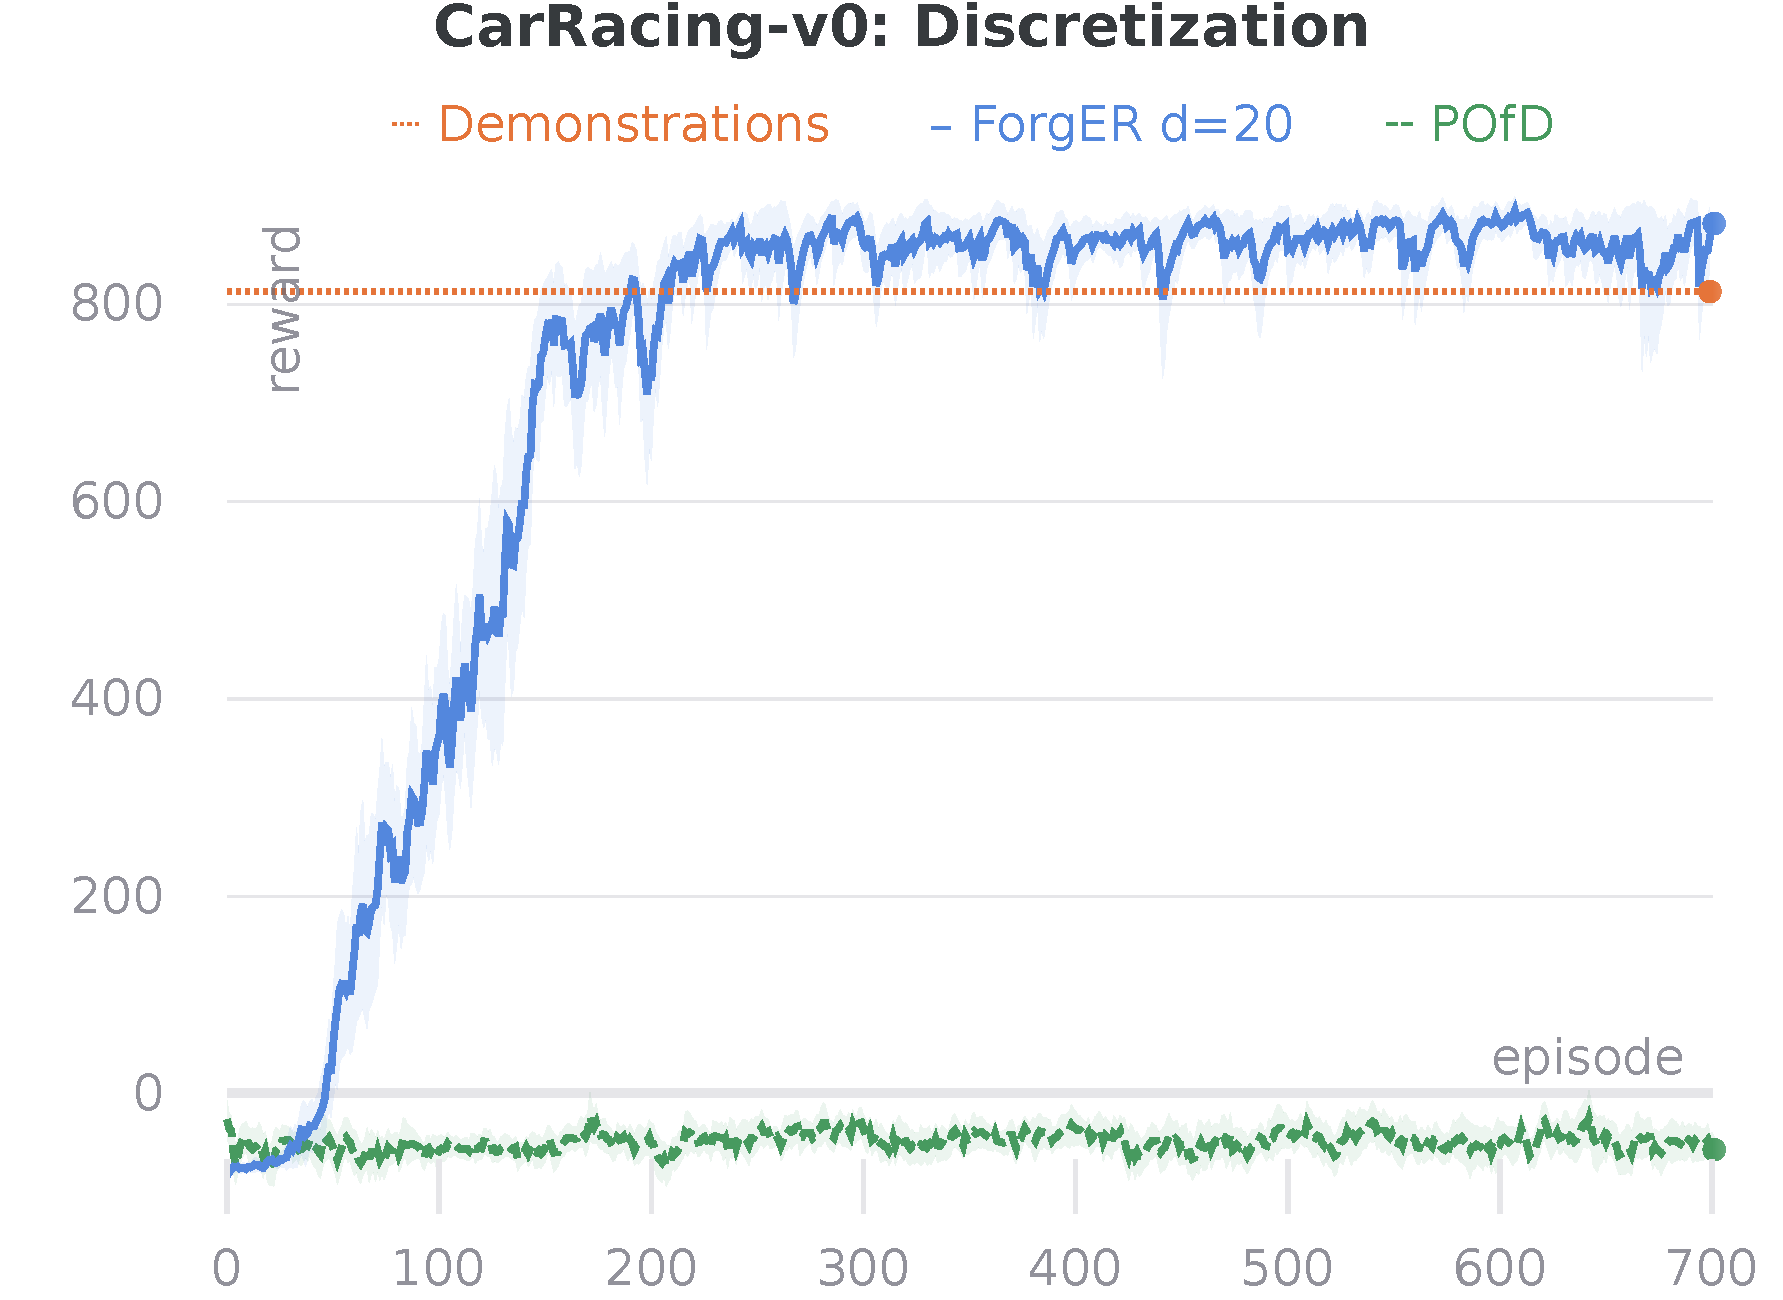
\includegraphics[width=0.48\linewidth]{img/discretization-lander-carracing/car.pdf}}

    \vspace{-0.2cm}
    \label{fig:exp:discrete:pofd}
    \caption{Сравнение алгоритмов на \textit{LunarLander} (\textbf{слева}) и \textit{CarRacing} (\textbf{справа})  с экспертными данными после дискретизации.}
\end{figure*}

\begin{figure*}[ht]
    \centering
    \subfigure{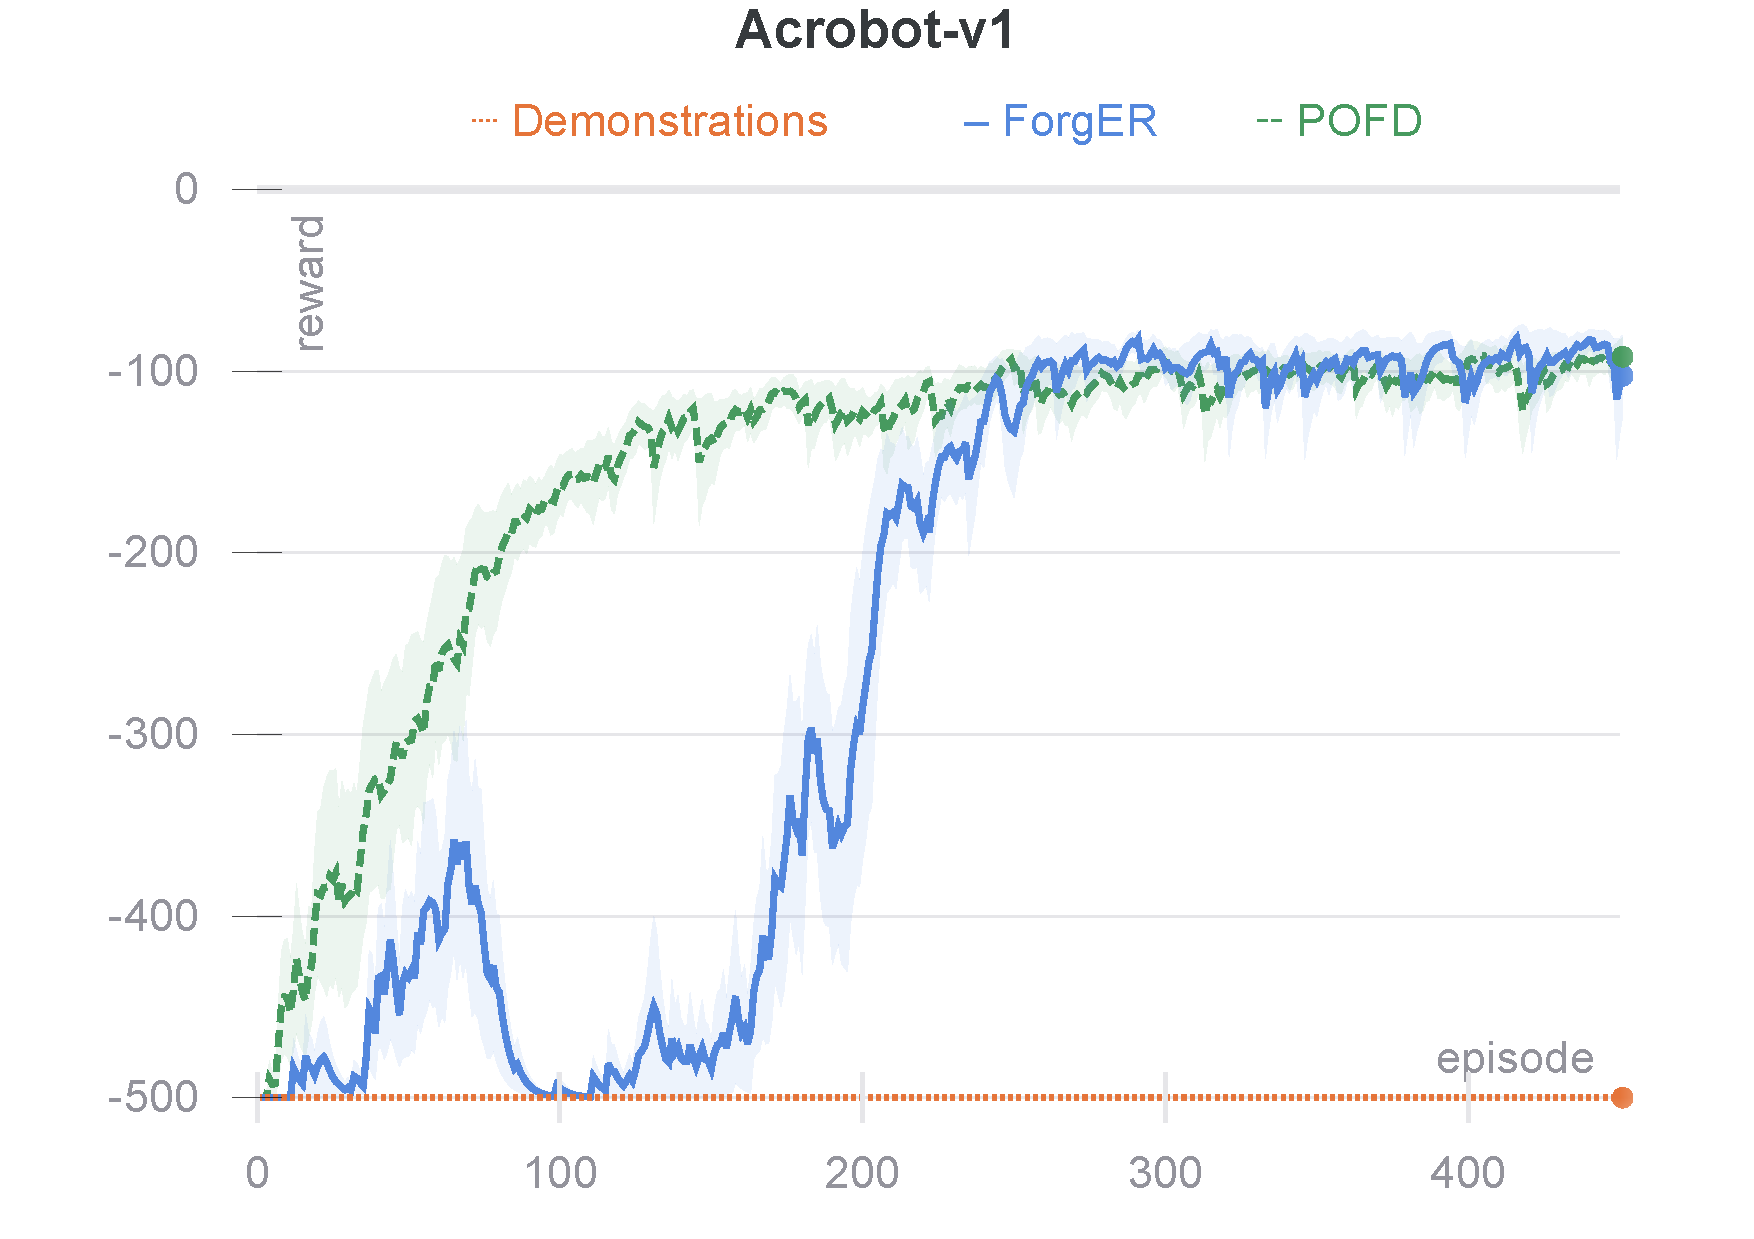
\includegraphics[width=0.48\linewidth]{img/classic-control/Acrobot-v1/a-e3.pdf}}
    \hspace{0.02\linewidth}
    \subfigure{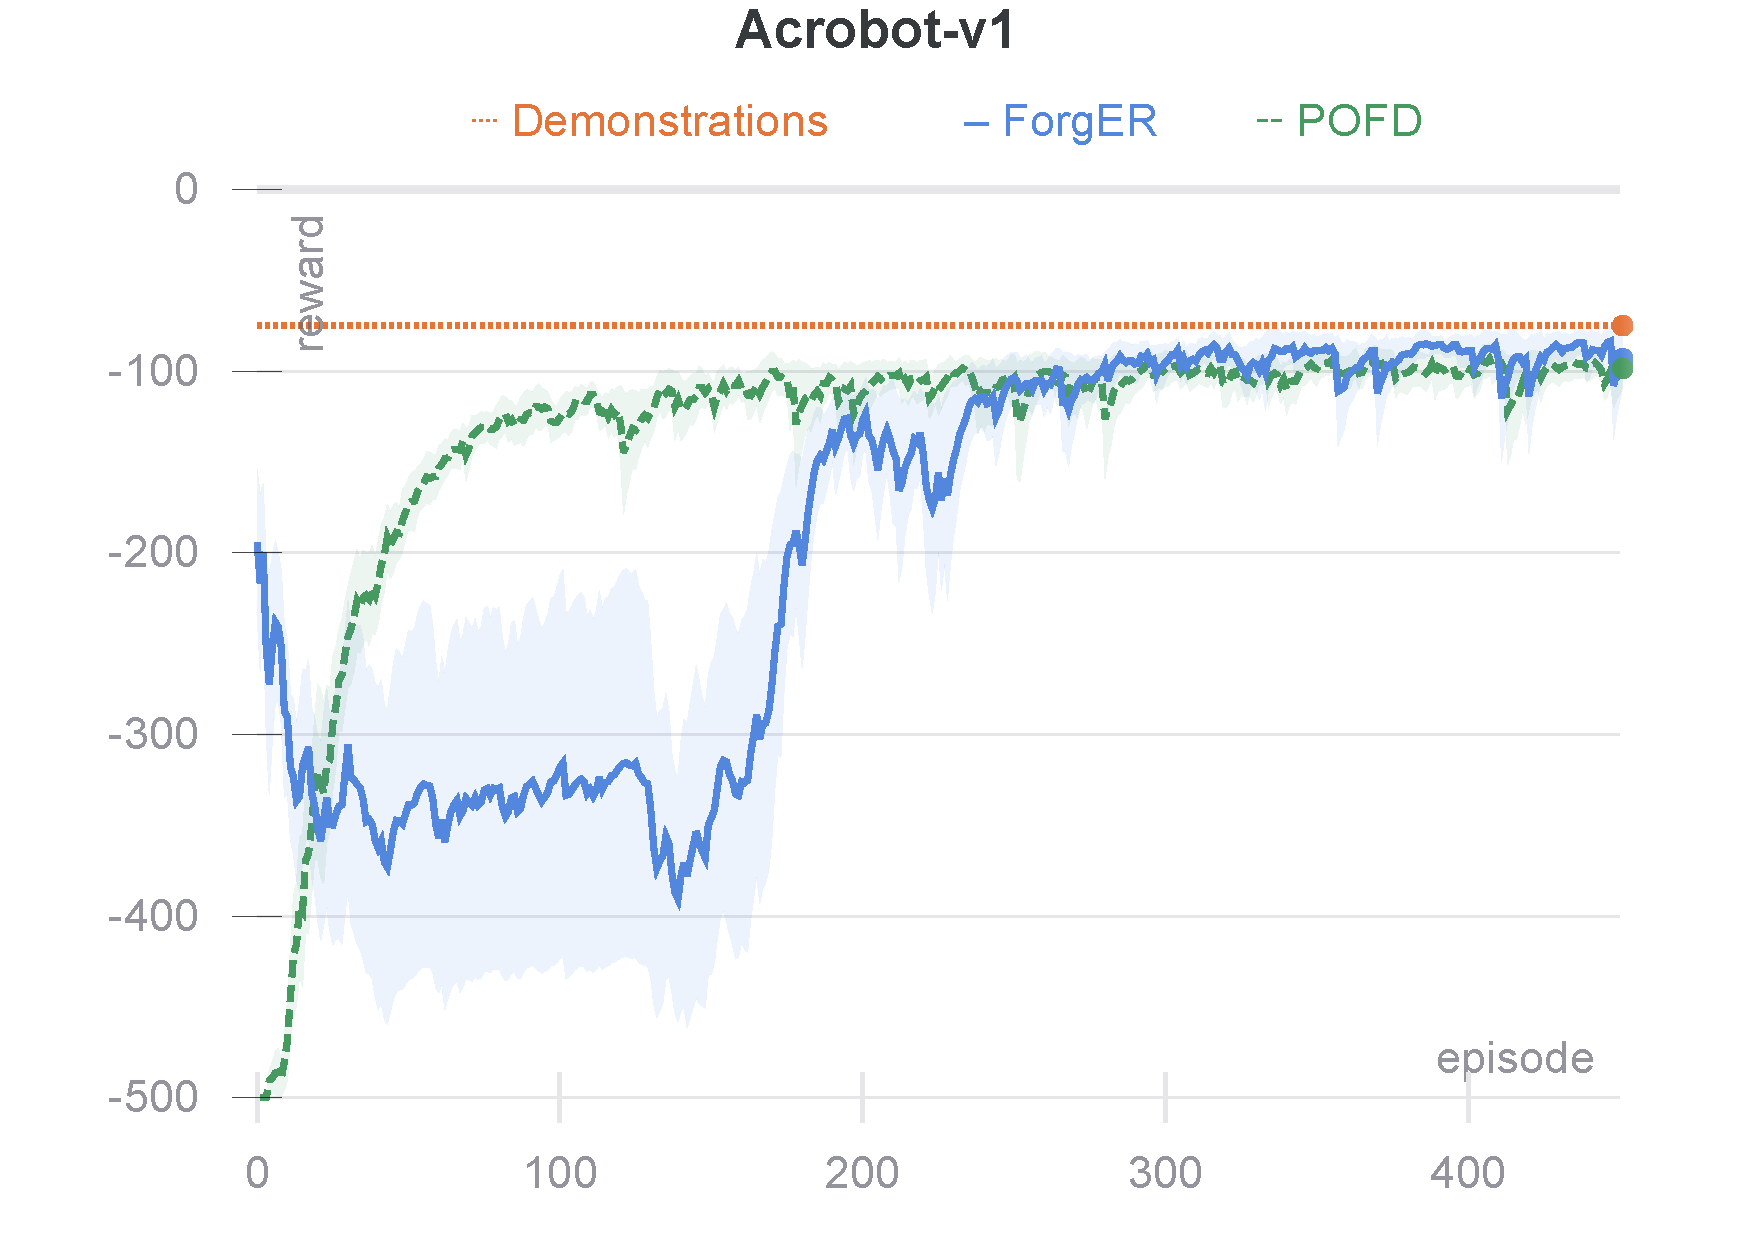
\includegraphics[width=0.48\linewidth]{img/classic-control/Acrobot-v1/a-e1.pdf}}
    \vspace{-0.2cm}
    \label{fig:exp:abot}
    \caption{Сравнение алгоритмов на среде \textit{Acrobot-v1}}
\end{figure*}

\begin{figure*}[ht]
    \centering
    \subfigure{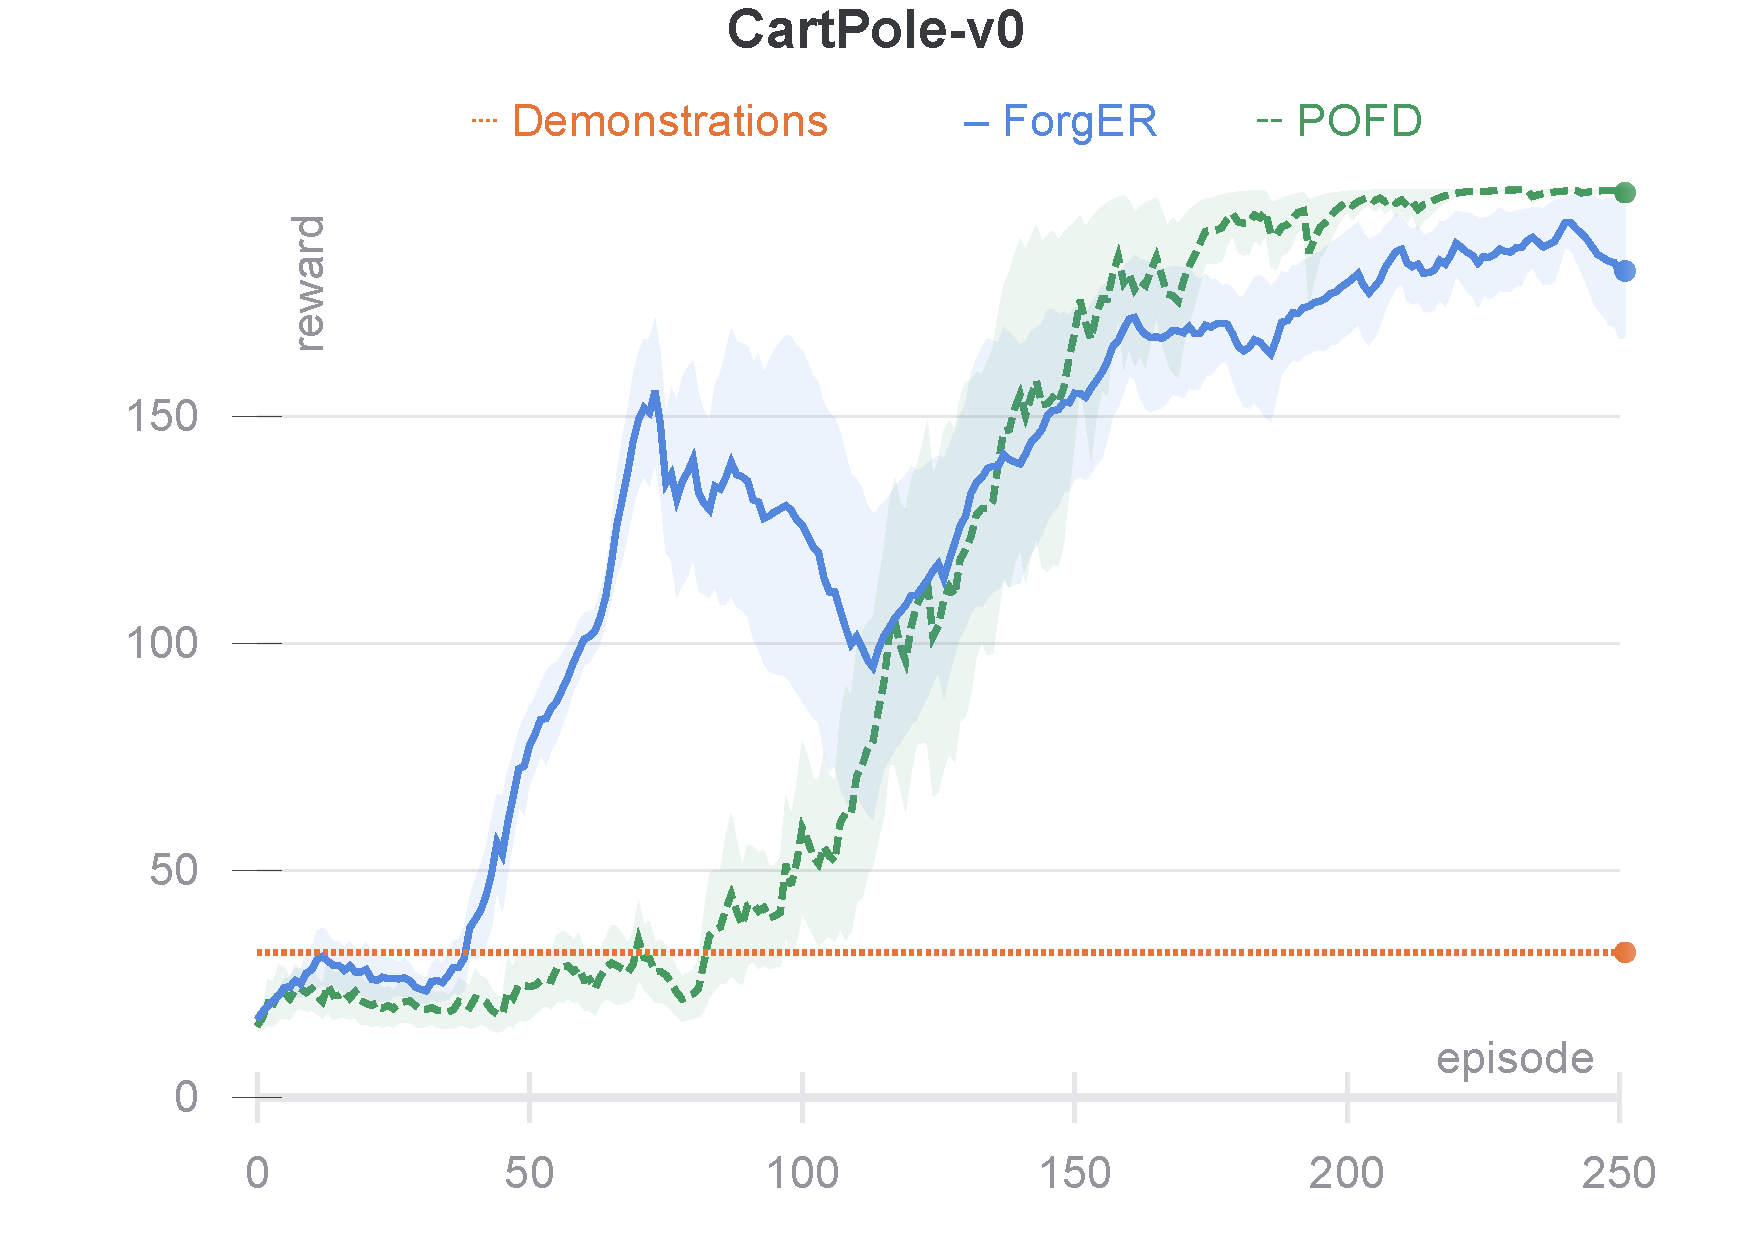
\includegraphics[width=0.48\linewidth]{img/classic-control/CartPole-v0/c-e3.pdf}}
    \hspace{0.02\linewidth}
    \subfigure{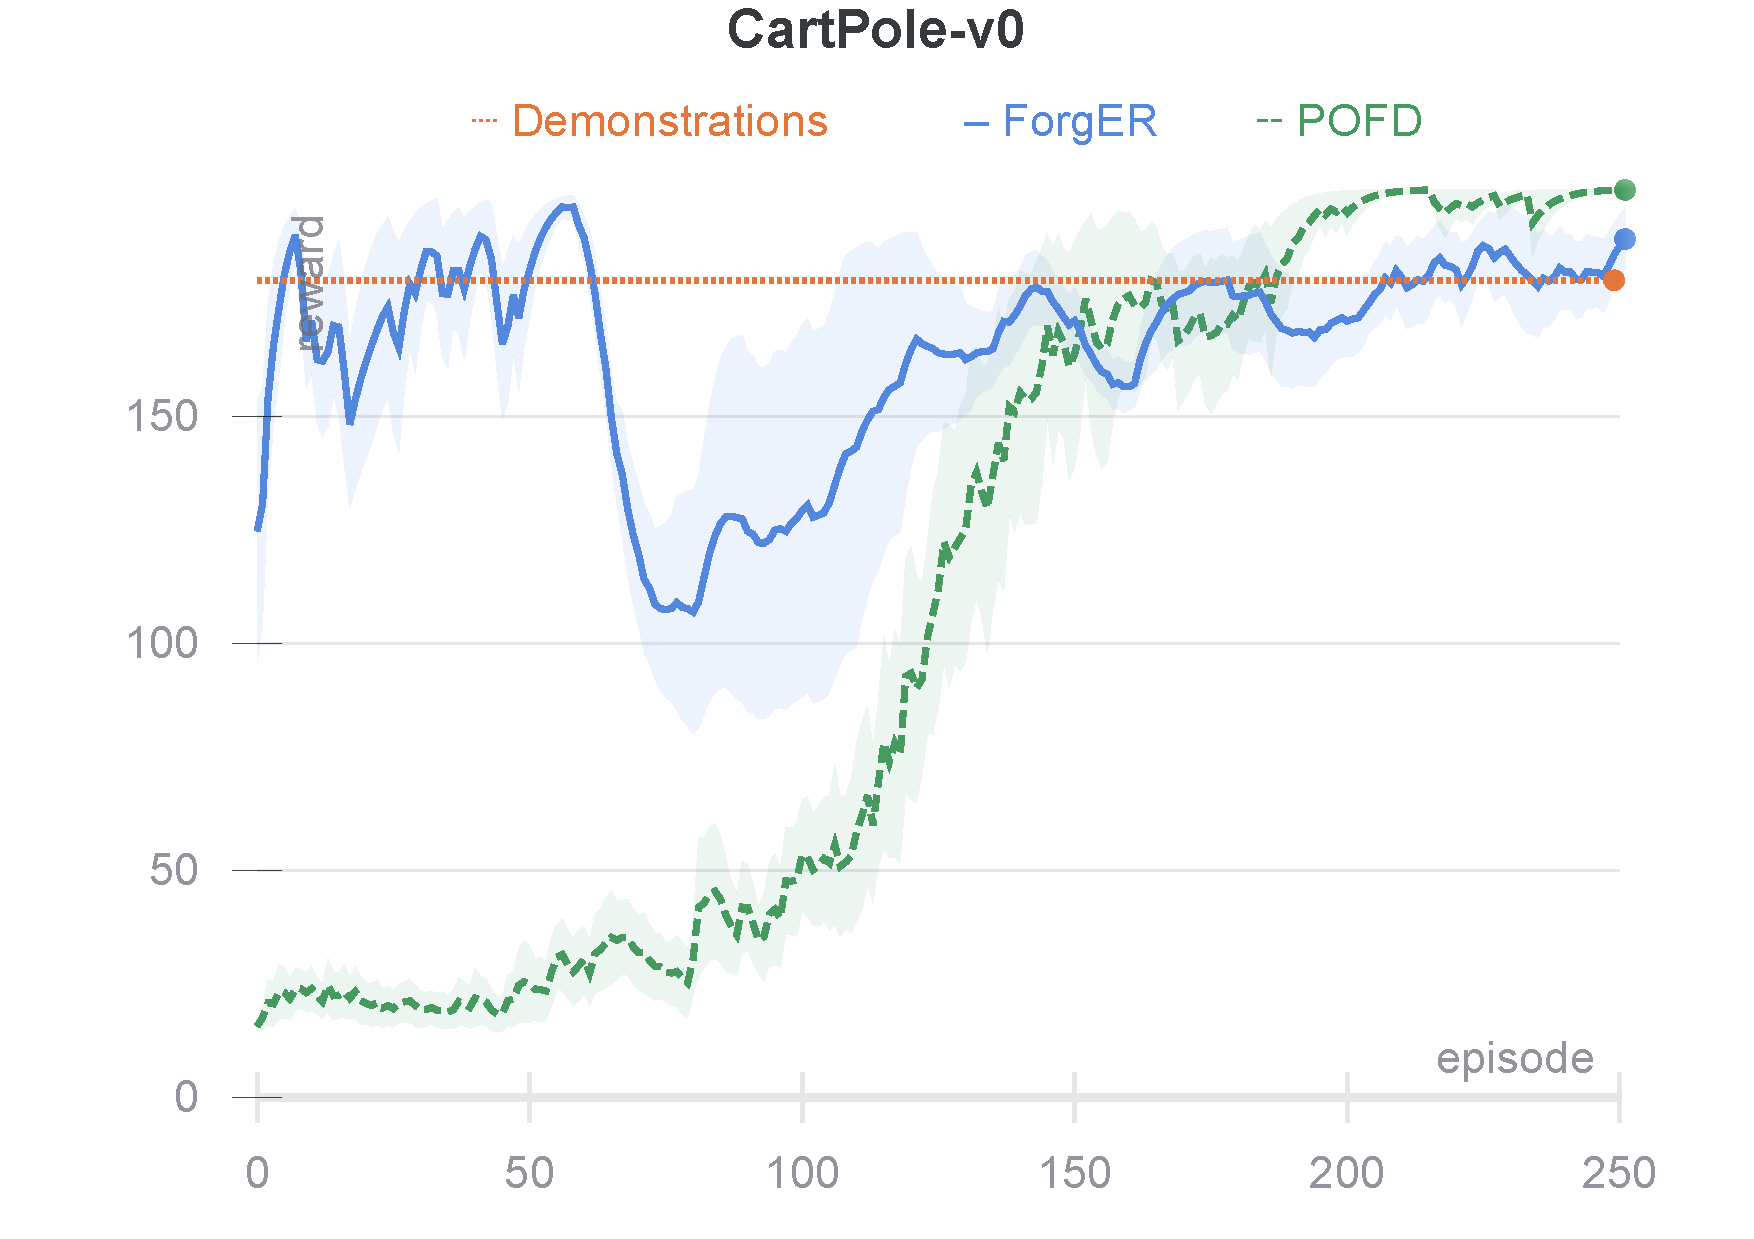
\includegraphics[width=0.48\linewidth]{img/classic-control/CartPole-v0/c-e2.pdf}}
    \vspace{-0.2cm}
    \label{fig:exp:cpole}
    \caption{Сравнение алгоритмов на среде \textit{CartPole-v0}}
\end{figure*}

\begin{figure*}[ht]
    \centering
    \subfigure{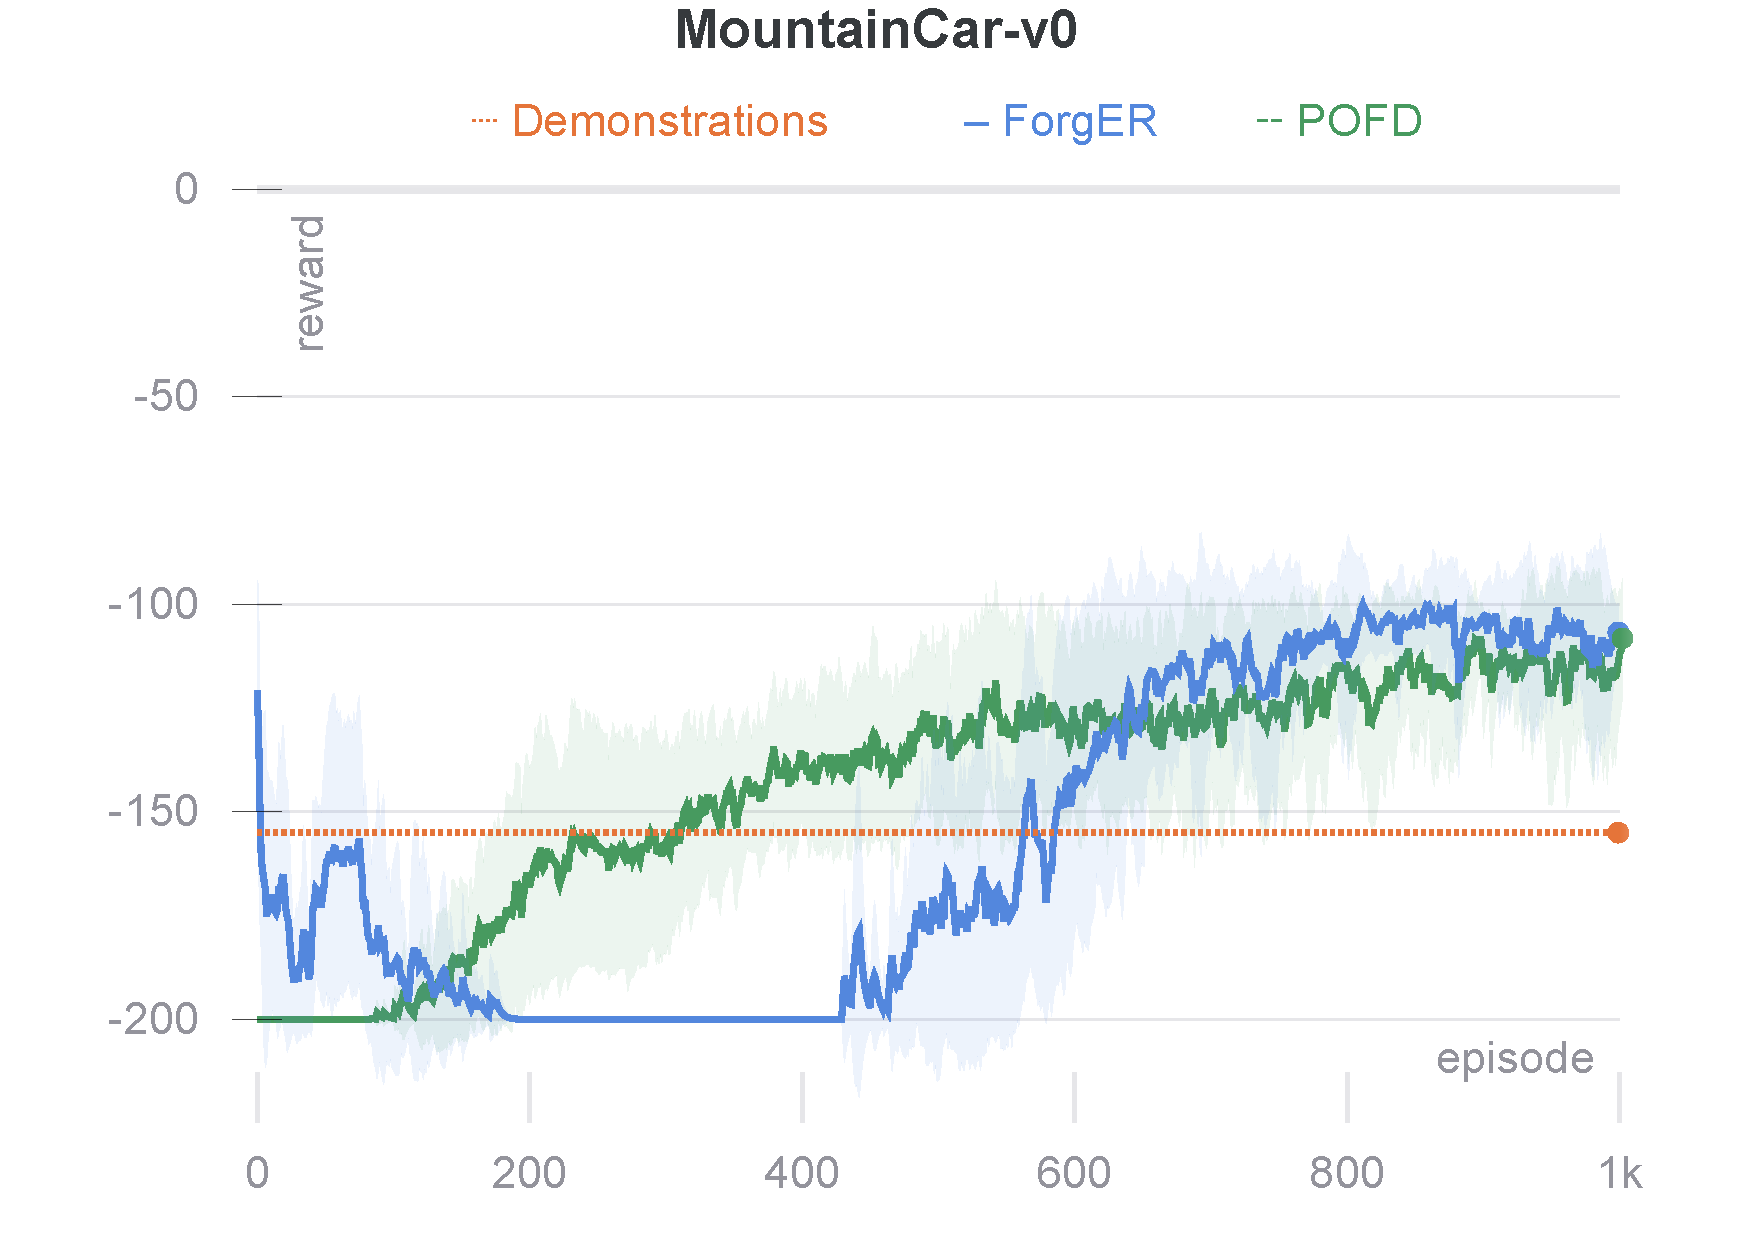
\includegraphics[width=0.48\linewidth]{img/classic-control/MountainCar-v0/m-e2.pdf}}
    \hspace{0.02\linewidth}
    \subfigure{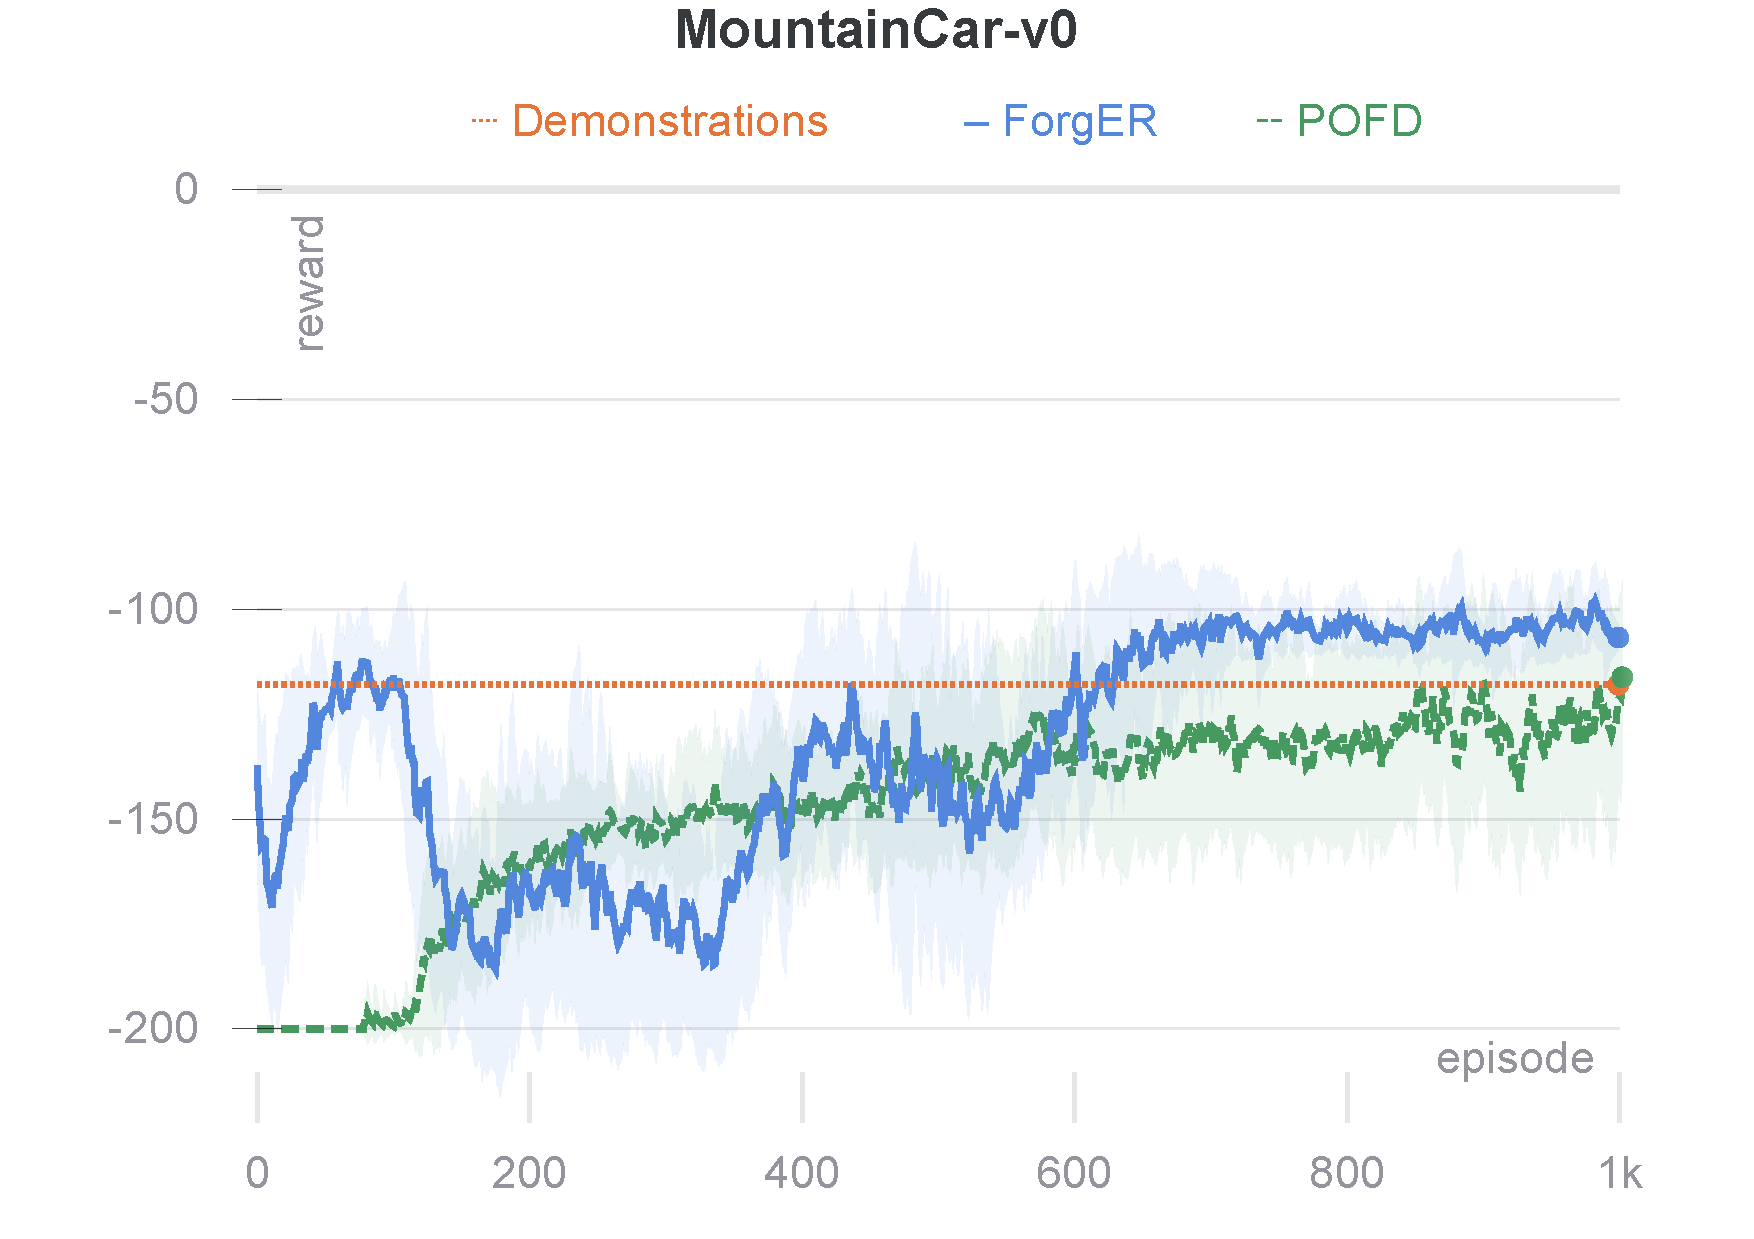
\includegraphics[width=0.48\linewidth]{img/classic-control/MountainCar-v0/m-e1.pdf}}
    \vspace{-0.2cm}
    \label{fig:exp:mcar}
    \caption{Сравнение алгоритмов на среде \textit{MountainCar-v0}}
\end{figure*}


\section{Окружающая среда \textit{RozumEnv}}

Для экспериментов с моделью робототехнического манипулятора Rozum в симуляторе CoppeliaSim была реализована среда \textit{RozumEnv} (рис. \ref{rozum}). Сцена симуляции представляет из себя стол с манипулятором и предметом перед ним. Управление производилось с помощью пакета \textit{PyREP} \cite{pyrep}, который в отличии от официального API предлагает более быстрое взаимодействие с языком программирования \textit{Python}. Окружение позволяет комбинировать разные пространства состояний: картинка/(картинка, положение манипулятора)/ (положение манипулятора, положение предмета). В качестве $r$ использовалась функция $tolerance$ из работы \cite{deepmind suite}, зависящей от расстояния манипулятора до предмета, и большой награды за захват предмета:
\begin{center}
$r(distance) = tolerance(distance, margin=0.25)/20 + \mathds{1}(grasped)\cdot 10$
\end{center}

Действия представляют из себя вектор углов \textit{joints} в сочленениях манипуляторов и действия по захвату \textit{ee}. Манипулятор производит сжатие если $ee\geq 0.5$ и разжатие если $ee< 0.5$. Действия в сочленениях выполнялись в течении 4 симуляционных шагов, а действия по сжатию и разжатию выполнялись до конца. Всего эпизод длился 200 симуляционных шагов, что представляет из себя 10 секунд (один симуляционный шаг составляет 0.05 секунд). В начале эпизода положение предмета выбирается случайным образом на площадке размером 20x15.

%картинка RozumEnv

\begin{figure*}[ht]
    \centering
    \subfigure{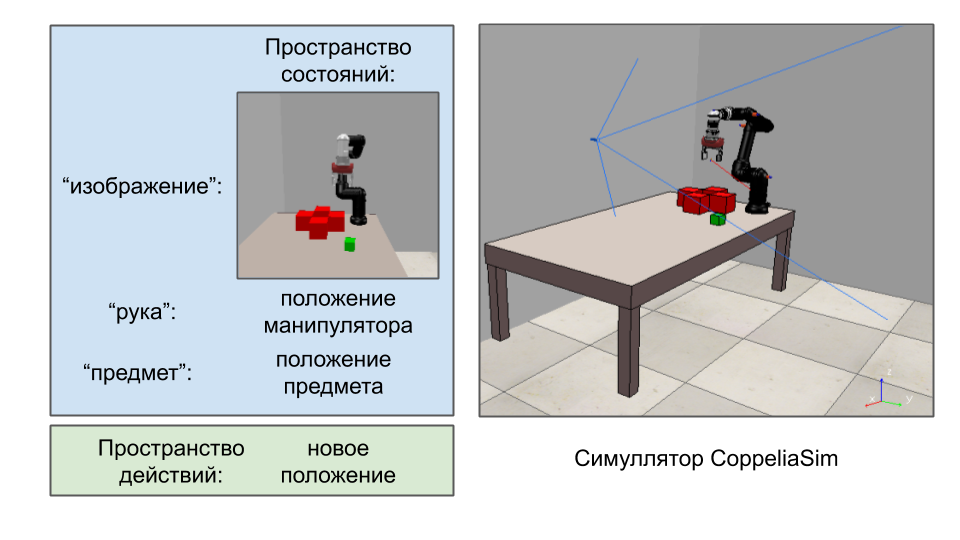
\includegraphics[width=0.8\linewidth]{img/RozumEnv.png}}
    \vspace{-0.2cm}
    \label{rozum}
    \caption{Окружающая среда \textit{RozumEnv}}
\end{figure*}

\section{Эксперименты в окружении \textit{RozumEnv}}

\backmatter

% \printbib
% Следующие строки необходимо раскомментировать, а предыдущую закомментировать, если используется inline-библиография.
\begin{thebibliography}{99}
    \bibitem{dqn}
        H. Mott-Smith, I. Langmuir. ``The theory of collectors in gaseous discharges''. \emph{Phys. Rev.} \textbf{28} (1926)
    \bibitem{ddpg}
        H. Mott-Smith, I. Langmuir. ``The theory of collectors in gaseous discharges''. \emph{Phys. Rev.} \textbf{28} (1926)
    \bibitem{Agent-57}
    \bibitem{OpenAI}
    \bibitem{DeepMind}
    \bibitem{vrep}
    \bibitem{apex}
    \bibitem{td3}
    \bibitem{Q-learning}
    \bibitem{double dqn}
    \bibitem{dueling dqn}
    \bibitem{per}
    \bibitem{n-step}
    \bibitem{polyak}
    \bibitem{dqfd}
    \bibitem{noisy layers}
    \bibitem{adaptive noise}
    \bibitem{pofd}
    \bibitem{deepmind suite}
    \bibitem{pyrep}
\end{thebibliography}

\chapter{Благодарности}

Благодарности идут тут.

\end{document}